\documentclass[autodetect-engine, dvipdfmx-if-dvi, ja=standard, 11pt]{bxjsreport}

\usepackage{subfiles}
\usepackage{pdfpages}
\usepackage{listings}
\usepackage{graphics}
\usepackage{float}

\lstset{
    basicstyle={\roboto},
    frame=tRBl,
    breaklines=true,
    framesep=10pt,
    linewidth=15cm,
    lineskip=-0.5ex,
    tabsize=2
}

\begin{document}

% 目次を追加
\tableofcontents

% 各章を追加
\begin{abstract}
    少人数のソフトウェア開発において,ビジネス要求を素早く実現するためにソースコードの追加・修正に追われ,
    ドキュメントの追加・修正を忘れてしまい,ソフトウェア品質を落としてしまうといった状況が見られる.
    これは,ソースコードからドキュメントを自動生成する技術を使用したり,ドキュメントとソースコードが乖離したときに開発者に通知を行うことで対応ができる.
    しかし,ソースコードからドキュメントを自動生成するためには,ライブラリやフレームワークに依存してしまうといった問題点があり,
    ドキュメントとソースコードが乖離したときに通知を行うためには手間がかかる問題点がある.
    
    以上より,ライブラリやフレームワーク,エディタに依存しない,ドキュメントとソースコードの乖離の可能性のある箇所の特定および通知を行うことのできるツールを開発した.
    ツールを利用するためには,CI/CDツールの設定ファイルに数行追加するだけでよいため,非常に軽量である.
    また,ツールの有効性を検証するために,Gitのコミット履歴を用いたシミュレータの開発および評価実験を行った.
    Pythonが使用されたOSSのプロジェクトを対象にシミュレーションを行ったところ,乖離リスクのある箇所に対して通知を行うといった結果が得られた.
    評価実験では,実験協力者2名に対し,前半5個,後半5個の合計10個のタスクをこなしてもらい,前後半のいずれかでツールが作動する実験を行った.
    このとき,ドキュメントとソースコードの乖離が抑制されるのかを評価の対象とした.
    また,実験終了後にアンケートを実施した.
    実験の結果,実験終了時にはドキュメントとソースコードが乖離することはなく,一定の効果が見込めることが判明した.
    また,アンケート結果から,「ドキュメントの更新を忘れてしまったとき,通知は必要である」といった回答を得ており,
    ドキュメントとソースコードの乖離抑制に役立つことができたと考えられる.
\end{abstract}
\chapter{序論}
近年のソフトウェア開発では,ソフトウェア開発における複雑性が増し,少人数の開発チームへと分割されていく中で,開発者は短期間でより多くの作業をしなくてはらならない状況にある.
そのため,分割されたチーム間で円滑な連携を行うことや,ソフトウェア品質を保つためにドキュメントを整備することが重要視されている\cite{maintenance}.
また,2020年初旬からの新型コロナウィルス感染症拡大により,ソフトウェア開発の現場ではリモートワークを中心としたテキストベースでのやり取りも増えたため,より一層ドキュメントを充実させる必要性が高まった.
このような状況において,開発スピードを求められるソフトウェア開発の現場では,ドキュメントとソースコードの整合性を維持することが困難となってきた.

ソフトウェア開発の現場では,バージョン管理システムを使用したソフトウェアのバージョン管理,CI/CD(継続的インテグレーション/継続的デリバリー)を活用したソフトウェアのビルド・テスト・デプロイの自動化,
円滑なやりとりを行うためのチャットツールの導入など,開発スピードの向上に力を入れている.
また,同じ開発チームであったとしても,フロントエンドの開発,バックエンドの開発,モバイルアプリケーションの開発,デザインの調整など開発者の役割は様々であり,
開発チームの内外問わずに円滑なやりとりを行う必要がある.
このため,ソフトウェア開発で使用するドキュメントは常に最新のものであることが求められている.

開発者は,ビジネス要求を素早く実現するために,機能の追加や修正を優先してしまい,ドキュメントの更新を後回しにしてしまう事例は少なくない.
例えば,誤って古いドキュメントを参照して開発を進めた場合,後の段階で手戻りが発生してしまうため,開発スピードを大幅に落としてしまう原因となってしまう.
また,普段と異なる開発環境では,開発者は自身の能力を最大限発揮することは難しい.
したがって,ライブラリやフレームワーク,エディタの制限を少なくし,既存のソフトウェア開発プロジェクトに無理なく組み込むことができるツールを作成する必要があると考えた.

以上を踏まえた上で,ドキュメントとソースコードの乖離している可能性のある箇所を特定および開発者に通知をすることができる機能をもった支援ツールを開発した.
これはライブラリやフレームワーク,エディタへの制限が少ないツールである.
同時に,ツールの有効性を検証するために,Gitのコミット履歴を使用したシミュレータの開発を行い,実際のソフトウェア開発を想定したシミュレーションを行った.
シミュレーションで検証できなかった機能については,実際にプログラミング経験が豊富な実験協力者にツールを使用してもらい,その有効性を確かめる評価実験を行った.

本論文の構成は以下のとおりである.2章で,本研究の関連研究について示し,本研究との相違点を述べる.
3章では本研究で提案するツールについて,4章ではその設計と実装について述べる.
5章では,提案ツールの有効性検証するためのシミュレーションおよび評価実験について述べる.
6章では,評価実験の結果と考察について述べ,7章で本研究の結論を述べる.
\chapter{関連研究}
本章では,本研究に関連する研究および技術と,本研究との相違点について述べる.

\section{ドキュメントとソースコードの一元管理}
赤石らの提案するドキュメントとソースコードの一元管理ツール\cite{seigousei}は,開発者がXML形式のドキュメントを作成した後,それに従ってソースコードを作成することで,ドキュメントとソースコードの整合性を維持すことを期待する.
作成したドキュメントとソースコードは,ビュワーを通じて閲覧を行うことができる.ビュワーではドキュメントとソースコードが混在した形で近い場所に表示されるため,開発者はドキュメントとソースコードの乖離に気づきやすい.
しかし,ドキュメントとソースコードの整合性を維持するためには,赤石らの提案するエディタおよびビュワーを使用しなくてはいけないため,開発者の学習コストや開発スピードの低下が懸念される.
また,ドキュメントとソースコードの対応付けを行う方法や,提案ツールの評価方法,ビュワーの見た目の調整が未実施である.

\section{ドキュメントとソースコードを対応付ける研究}
後藤らのドキュメントとソースコードの対応付けを行う研究\cite{taiouduke}では,ドキュメントをXML形式で記述したものを扱い,
XMLのタグとソースコード中の識別子を対応表を用いて対応付けを行う.これによって,ドキュメントとソースコードの整合性を検査できるようになった.
しかし,ドキュメントまたはソースコードのどちらかの編集に対して,インタラクティブな機能を提供することができず,
例えば,先にドキュメントを作成してからソースコードを記述する方法では不整合として扱われてしまうといった問題点がある.

\section{ドキュメントからソースコードを生成する研究}
小池のドキュメントからソースコードを生成するフレームワークSLAF\cite{framework}では,ドキュメントとソースコードの乖離の発生は防げないといった考えから,
ドキュメントからソースコードを生成することができる.
具体的には,プログラミング言語の知識を必要としないドキュメントを記述することで,それに従って動作するJavaのソースコードが生成される.
これによって,常にドキュメントとソースコードの整合性が維持されることになった.
しかし,生成されたソースコードでは性能低下が見られることや,現実的に運用することが難しいといったことから課題も多い.

海老澤らのWebComponents開発におけるAPIドキュメントとソースコードを自動生成する研究\cite{webcomponents}では,
1つのファイルに,HTML, CSS, JavaScriptとAPIドキュメントを記述することで,ドキュメントとソースコードを同時に管理することのできるシステムを開発した.
これは,既存のシステム開発に組み込むことは難しく,新たなプロジェクトで有効に作用すると考えられる.

丹野らのソフトウェアの設計ドキュメントからソフトウェアテストを行うコードを生成する研究\cite{test}では,
仕様や設計の変更に強いといった利点があり,ドキュメントとソフトウェアの整合性を維持することができる.
しかし,Webアプリケーションのみに利用可能であることや,開発手法にウォーターフォール型開発を採用しなくてはならないため,使用用途が限定されてしまうといった問題がある.

\section{ソースコードからドキュメントを生成する研究}
Boyangのソースコードからドキュメントを生成する研究\cite{automatically}では,
ソースコードと単体テストのテストケースを解析し単体テストに関する説明をまとめたドキュメントを自動生成するシステムと,
ソースコードとデータベースのスキーマを解析しデータベースの操作およびスキーマが記述されたドキュメントを自動生成するシステムを提案している.
これにより,ソフトウェア開発を円滑に行うことができるようになった.
しかし,プロジェクトの方針やアーキテクチャ,概要機能の設計には対応していないため,これらを記述するドキュメントは提案システムを使用せずに作成する必要がある.

\section{ソースコードからドキュメントを生成する技術}
ソースコード中に適切なアノテーションやコメント文を挿入することで,ドキュメントを自動生成することのできるライブラリやフレームワークが存在する.
それぞれのライブラリやフレームワークでドキュメントを自動生成するための書き方は異なるが,いずれも適切な箇所で適切なフォーマットでコーディングする必要がある.
以下では,ドキュメントを自動生成することができるライブラリおよびフレームワークを紹介する.

\subsection{Javadoc}
Javadoc\cite{javadoc}は,JDKに標準搭載された機能で,適切なフォーマットに従って作成したコメント文やソースコードからHTML形式のドキュメントを自動生成するツールである.
プログラミング言語にJavaを使用したソフトウェア開発では,ソースコードのAPI仕様書としてにJavadocが使用されることも多い.
Javaのソースコードからドキュメントを生成するため,例えば,プロジェクトの方針やアーキテクチャ,概要機能の設計を記述するドキュメントには不向きである.


\subsection{Spring Boot}
Spring Boot\cite{spring}は,Webアプリケーション開発を行うことのできるJavaのWebフレームワークである.
RESTful APIを実装するときに,Swagger\cite{swagger}と呼ばれるドキュメントを自動生成する機能が存在する.
Javaで記述するソースコード中に適切な箇所で適切なアノテーションを埋め込むことで,ソースコードから自動でドキュメントを生成することができる.

\subsection{FastAPI}
FastAPI\cite{fastapi}は,APIサーバーを構築することのできるPythonのWebフレームワークである.
FastAPIにはSwaggerとReDoc\cite{redoc}と呼ばれるドキュメントを自動生成する機能が存在する.
Spring Bootと同様に,ソースコード中に適切な箇所で適切なアノテーションを埋め込むことで,ソースコードから自動でドキュメントを生成することができる.
また,追加のプラグインやライブラリを必要とせずに,元からある機能として組み込まれているため,簡単に利用することができる.
しかし,SwaggerやReDoc以外のドキュメントを生成することができないため,その他ドキュメントに関しては,開発者が意識して,ドキュメントとソースコードの整合性を維持しなくてはならない.

\section{本研究との相違点}
赤石らの研究で提案されたドキュメントとソースコードの一元管理を行うツールでは,目的は同じであるものの,プログラミング言語やエディタが限定されるのに対し,
本研究では,ライブラリやフレームワーク,エディタへの制限が少なく,既存のソフトウェア開発プロジェクトに無理なく組み込むことができるといった点で異なる.
また,その他関連研究やドキュメントを自動生成するライブラリやフレームワークでは,技術選定の段階で制限されてしまうのに対し,本研究では,現在進行中のプロジェクトに無理なく組み込むことができるといった点で異なる.
ただし,本研究で提案する全ての機能を使用するためには,ライブラリやフレームワークを指定する必要があることに留意する.
プロジェクトに使用されるライブラリやフレームワークに応じて,適切な機能を選択しなくてはならない.

また,ドキュメントを自動生成することができるライブラリやフレームワークでは,ソースコードに直接関係のないドキュメント,例えば,開発プロジェクトのアーキテクチャの概念図やプロジェクトの方向性,
補助的な説明を記載するドキュメントは,通常ソースコード中には記載せずに,別途ドキュメント専用のファイルに記載するため,自動生成がすべてをカバーできないことに留意する.
これらのドキュメントも,プロジェクトが進み古くなってしまうと,ドキュメントとソースコードが乖離してしまう可能性がある.

本研究ではドキュメントとソースコードが乖離している可能性のある箇所を特定および開発者に通知をすることができる機能をもったツールの開発を行う.

\chapter{提案手法}
本章では,本研究で提案するツールについて述べる.

\section{想定利用者}
1章で述べたとおり,ソフトウェア開発のチームでドキュメントとソースコードの乖離を抑制することが目的なため,
ソフトウェア開発を行う少人数(3名〜6名程度)の開発チームを対象としている.
大人数で行うソフトウェア開発では,プロジェクトで使用する技術やツールの自由度が制限されることが多いことや,
少人数のソフトウェア開発チームに分割されていくことを踏まえて,提案ツールは少人数のソフトウェア開発に焦点を当てて開発した.

\section{提案ツール}
\label{tool}
本節では,提案ツールの目的,要求仕様について述べる.

\subsection{提案ツールの目的と要求仕様}
\label{required}
提案ツールの役割は,ドキュメントとソースコードの乖離リスクのある箇所を特定し,開発者への通知を行ったときに,通知内容をもとに開発者がドキュメントまたはソースコードを修正することで,乖離を抑制することを期待する.
また,既存のソフトウェア開発に無理なく組み込むことができるようにするために,ライブラリやフレームワーク,エディタへの制限が少なくなるように設計する.
これを実現するためにツールには以下の機能をもたせる.このとき,それぞれの機能にC1〜C4と名付けた.
いずれの機能も,リモートリポジトリであるGitHub上にプッシュされた際に,CI/CDツール上で動作するツールが乖離リスクを検知する仕組みとなっている.
また,C1〜C4の機能について,開発者がパラメータを自由に変更できるようにし,パラメータを変更する際はコミュニケーションツールを通じて行う.
現状では,Slackのコマンドを利用してパラメータを変更できるように実装しているが,他のコミュニケーションツールのAPIを適切に利用することで,切り替えることも可能である.

\subsection{C1:ソースコード先行の検知の機能}
\label{c1}
アノテーションを用いてドキュメントとソースコードの対応付けを行い,ドキュメント中に記述されていない機能をソースコードに実装した際に,乖離リスクとして開発者に通知する.
本機能は,RESTful APIの開発に利用可能であり,プログラミング言語にPython,ドキュメントにSwaggerを選択する必要がある.
現状では,プログラミング言語にPythonを使用しなくてはならないが,提案ツールから他のプログラミング言語の呼び出しを行い,静的解析を行うことで,他のプログラミング言語も利用することができるようになる.
開発者は,この通知を受け取ったときに,ドキュメントに適切なものを追加するか,誤ったアノテーションを修正し,ドキュメントとソースコードの乖離を抑制することを期待する.

具体的な仕組みについて,FastAPIを使用したRESTful APIのソースコード\ref{c1code}と,Swaggerのドキュメント\ref{c1doc}を例にまとめる.
これは,GETメソッドで/usersにHTTPリクエストを送信すると,ユーザーの一覧取得を行うことのできるRESTful AIPのソースコードとドキュメントである.
Swagger形式のドキュメントは,JSONまたはYAMLで記述することができる.
ドキュメント中のoperationIdはオプション値であり,エンドポイント毎にユニークな値を設定する必要がある.
また,機能となる関数の上部(FastAPIではデコーレータである@appの上部)に,コメントアウトで@operationIdと記述することで,ドキュメントとソースコードの対応付けを簡単に行えるようになる.

\begin{lstlisting}[caption=RESTful API, label=c1code]
# @operationId get_users
@app.get('/users')
def get_users():
    response = []

    for user in get_users_from_db():
        response.append({
            'user_id': user.user_id,
            'name': user.name,
            'age': user.age
        })

    return response
\end{lstlisting}


\begin{lstlisting}[caption=Swagger,label=c1doc]
"paths": {
     "/users": {
         "get": {
            "summary": "Get a list of users.",
            "operationId": "get_users",
            "responses": {
                "200": {
                    "description": "Successfully get the list of users."
                }
            }
        }
    }
}
\end{lstlisting}

以下に,C1で変更可能なパラメータについてまとめる.
\begin{description}
    \item[C1a:ドキュメントの拡張子] C1機能で利用するSwaggerドキュメントの拡張子(現状では.jsonのみ利用可能)
    \item[C1b:ソースコードの拡張子] C1機能で利用するソースコードの拡張子(現状では.pyのみ利用可能)
\end{description}


\subsection{C2:一定時間経過後のリマインダーの機能}
\label{c2}
ドキュメントが作成され一定時間経過した後,ソースコードは更新され続けているがドキュメントは更新されていない場合に,乖離リスクとして開発者に通知する.
本機能は,ドキュメントとソースコードが同じリポジトリで管理されることを想定している.
また,Markdown形式ファイルやreStructuredText形式ファイル,単純なテキストファイルをドキュメントとして同一のリポジトリで管理する利用する必要がある.
開発者は,この通知を受け取ったときに,ドキュメントが古くなっていないかを確認し,古くなった箇所を修正するか,または現状維持でよいのかを判断し,ドキュメントとソースコードの乖離が抑制されることを期待する.

以下に,C2で変更可能なパラメータについてまとめる.
\begin{description}
    \item[C2a:経過日数] ドキュメントが更新されないことを通知するために必要な経過日数
    \item[C2b:ドキュメントの拡張子] C2機能で利用するドキュメントの拡張子(自由に設定可能)
    \item[C2c:ソースコードの拡張子] C2機能で利用するソースコードの拡張子(自由に設定可能)
\end{description}

\subsection{C3:リリース時ドキュメント更新有無の検知の機能}
\label{c3}
新たなバージョンがリリースされたとき,前回のバージョンリリース時よりドキュメントが更新されていない場合に,乖離リスクとして開発者に通知する.
本機能は,一定時間経過後のリマインダーの機能と同様に,ドキュメントとソースコードが同じリポジトリで管理されていることを想定している.
開発者は,この通知を受け取ったときに,前回のバージョンリリース時との変更点をドキュメントに記述するか,または現状維持でよいのかを判断し,ドキュメントとソースコードの乖離を抑制することを期待する.

具体的な仕組みについて,Pythonのパッケージ管理およびバージョン管理を行うソースコード\ref{c3version}のsetup.pyを例にまとめる.
これには,Pythonファイルにプロジェクト名である「management-system」と,そのバージョンは0.0.1が記述されている.
ここに記述されているversionを読み取り,C3の機能として利用する.
その他,例えばJavaScriptやTypeScriptのプロジェクトで使用されるpackage.jsonでは,JSONファイルにプロジェクト名やバージョンを記載する.
現状では,setup.pyのみ利用可能であるが,他のプログラミング言語のパッケージ管理ツールやバージョン管理ツールの解析を行うことで,拡張することができるようになる.

\begin{lstlisting}[caption=setup.py, label=c3version]
from setuptools import setup

setup(
    name='management-system',
    version='0.0.1'
)    
\end{lstlisting}

以下に,C3で変更可能なパラメータについてまとめる.
\begin{description}
    \item[C3a:バージョン管理を行うファイルのパス] バージョン管理を行うファイルの相対パス(現状ではsetup.pyのみ利用可能)
    \item[C3b:ドキュメントの拡張子] C3機能で利用するドキュメントの拡張子(自由に設定可能)
    \item[C3c:ソースコードの拡張子] C3機能で利用するソースコードの拡張子(自由に設定可能)
\end{description}

\subsection{C4:ソースコード変更量の検知の機能}
\label{c4}
新たなファイルを作成,既存のファイルを変更・削除したとき,ある一定量の変更が行われた場合に,乖離リスクとして開発者に通知する.
本機能は,一定時間経過後のリマインダーの機能と同様に,ドキュメントとソースコードが同じリポジトリで管理されていることを想定している.
開発者は,この通知を受け取ったときに,ドキュメントが古くなっていないかを確認し,古くなった箇所を修正するか,または現状維持でよいのかを判断し,ドキュメントとソースコードの乖離を抑制することを期待する.

以下に,C4で変更可能なパラメータについてまとめる.
\begin{description}
    \item[C4a:ソースコードの変更量] ソースコードの追加・削除・変更によって通知を送るのに必要な変更量
    \item[C4b:ドキュメントの拡張子] C4機能で利用するドキュメントの拡張子(自由に設定可能)
    \item[C4c:ソースコードの拡張子] C4機能で利用するソースコードの拡張子(自由に設定可能)
\end{description}
\chapter{設計と実装}
本性では,提案ツールおよび提案ツールを動作するシミュレータについて述べる.

\section{開発環境}
提案ツールの開発環境を下記に示す.

\begin{itemize}
    \item OS:macOS Big Sur 11.1
    \item プログラミング言語:Python 3.7
    \item 統合開発環境:PyCharm 2020.3.2
\end{itemize}

\section{提案ツールのアーキテクチャ}
\label{toolartchitecture}

\begin{figure}[H]
    \centering
    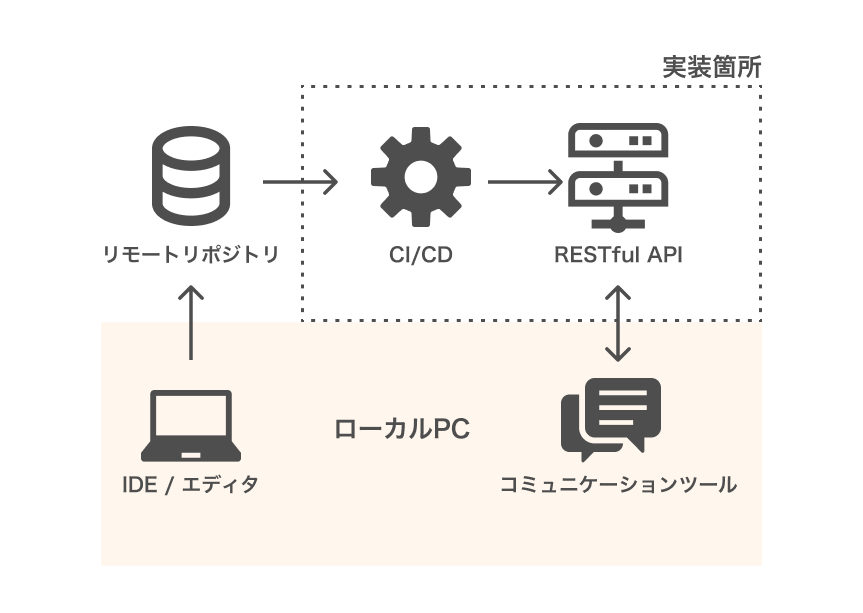
\includegraphics[width=12cm]{images/architecture.png}
    \caption{提案ツールのアーキテクチャ}
    \label{architecture}
\end{figure}

提案ツールのアーキテクチャを図\ref{architecture}に示す.
提案ツールは,既存のCI/CDツール上で動作することを想定しており,本研究ではCI/CDツールにGitHub Actionsを用いた.
また,CI/CDツール上で乖離の検知を行うが,できることが限られているため,同時に,Slackとのやりとりや,開発プロジェクトの状態の管理を行うことができるRESTful APIの開発も行った.
RESTful APIにはFastAPIを使用し,各種データの保持はJSONファイルにて管理を行っている.
また,RESTful APIは筆者のローカルPC上で動作させているが,HTTPSとして外部公開させることができるツールのngrokを使用しており,
Slack APIやCI/CDツール上で動作する提案ツールは,ローカルPC上で動作するRESTful APIを使用できるようになっている.

RESTful APIには,下記の機能をもたせているが,乖離検知の処理はすべてCI/CDツール上で動作するツールで行う.
\begin{itemize}
    \item 各機能のステータスを更新する機能
    \item Gitのコミットの差分量を追加する機能
    \item SlackのAPIを呼び出してメッセージを送受信する機能
\end{itemize}

Slackからに入力したコマンドをRESTful APIに反映させるための手順を下記にまとめる.
\begin{enumerate}
    \item Slackにコマンドを入力する
    \item Incoming Webhookより,SlackからRESTful APIに入力したコマンド内容がPOSTで送信される
    \item RESTful APIでは,受け取ったコマンドを解析し,適切な処理を行う
    \item 必要があれば,Slackにメッセージを送信する
\end{enumerate}

また,乖離検知を行い,検知した内容をSlackへと送信するための手順を下記にまとめる.
\begin{enumerate}
    \item GitHubへのプッシュを検知し,CI/CDツールが起動する
    \item CI/CDツール上で乖離検知を行うために,必要なデータをRESTful APIから取得する
    \item 取得したデータをもとに,乖離検知を行う
    \item 乖離検知をした場合,検知した内容を整形してメッセージとしてまとめ,RESTful APIにPOSTリクエストを行う
    \item RESTful APIからSlackにメッセージを送信する
\end{enumerate}

\section{提案ツールの使用方法}
開発者は,適切なタイミングで変更を記録するためにコミットを実行し,リモートリポジトリにプッシュすることを期待している.
\ref{toolartchitecture}節にまとめたとおり,提案ツールはリモートリポジトリにプッシュされたタイミングで,CI/CDツールが起動し,CI/CDツールの設定ファイルに定義されたコマンドに従って実行される.
そのため,提案ツールはGitHub Actionsを利用可能な状況ではローカルPCに専用の環境を構築せずに利用することができる.
ただし,提案ツールを利用するにあたっていくつか準備が必要であるため,それについてまとめる.
まず,CI/CDツール上で動作させるために,プロジェクトのディレクトリにtoolsディレクトリを作成し,そのディレクトリの中にPythonで作成された提案ツールを配置する.
CI/CDツールの設定ファイルには,プッシュ時に提案ツールを実行するように記述するだけでよい.
次に,SlackのAPIページより,提案ツールを登録する必要がある.
最後にRESTful APIの動作環境を用意する必要がある.例えばGCP(Google Cloud Platform)やHerokuなどのPaaS(Platform as aa Service)を利用することで,RESTful APIを動作する環境を用意することができる.
筆者が作成したRESTful APIをSaaSとして展開し,数多くのプロジェクトで利用することもできるが,現状ではセキュリティ上の懸念から各プロジェクトでRESTful APIを構築するのが望ましい.
いずれも,各Webサービスの登録手順に従って進めていくだけでよく,PaaSをよく理解していればRESTful APIの実行環境を簡単に構築することができる.

\section{コミュニケーションツールで利用可能なコマンド}
milkでは,Slackのスラッシュコマンドを活用することで,各種パラメータの設定を行うことができるようになっている.
以下では,milkで使用可能なコマンドをまとめる.

\subsection*{/milk c1 doc [ file type ]}
ソースコード先行検知の機能において,開発プロジェクトで使用するSwaggerドキュメントのファイル形式を指定することができるコマンドである.
本コマンドは,開発プロジェクトの初期段階でSwaggerドキュメントのファイル形式を指定する場合や,開発プロジェクトの途中でファイル形式を変更したい場合に利用されることを想定している.

\subsection*{/milk c1 code [ file type ]}
ソースコード先行検知の機能において,開発プロジェクトで使用するプログラミング言語を指定することができるコマンドである.
現在では,プログラミング言語にPythonのみを指定可能である.

\subsection*{/milk c1 param}
ソースコード先行検知の機能において,現在設定しているSwaggerドキュメントの拡張子および使用しているプログラミング言語の拡張子を確認することができるコマンドである.

\subsection*{/milk c2 set [ days ]}
一定時間経過後のリマインダーの機能において,ドキュメントが更新されずソースコードのみが更新されている場合に,ドキュメントを追加・修正するためのリマインダーを行う間隔を指定することができるコマンドである.

\subsection*{/milk c2 param}
一定時間経過後のリマインダーの機能において,現在設定しているリマインダーを行う間隔を確認することができるコマンドである.

\subsection*{/milk c3 set [ version file ]}
リリース時ドキュメント更新有無の検知の機能において,バージョンを扱うファイルを指定することができるコマンドである.
例えば,Pythonではsetup.pyと呼ばれるファイルにソフトウェアのバージョンを記述している.
現在では,バージョンを扱うファイルにsetup.pyのみを指定可能である.

\subsection*{/milk c3 param}
リリース時ドキュメント更新有無の検知の機能において,現在設定しているバージョンを扱うファイルを確認することができるコマンドである.

\subsection*{/milk c4 set [ number ]}
ソースコード変更量の検知の機能において,ドキュメントが更新されずソースコードのみが更新されている場合に,ソースコードの追加・削除・修正が行われた行数を指定することができるコマンドである.
指定した行数を超過してソースコードのみを記述し続けたときに通知がでる.

\subsection*{/milk c4 param}
ソースコード変更量の検知の機能において,現在設定している変更量を確認することができるコマンドである.

\section{シミュレータの設計}
シミュレーションには,CI/CDツール上で動作する乖離検知機能の一部を利用した.
シミュレーションの実行結果をグラフに描画するにあたり,Pythonのグラフ描画ライブラリであるMatplotlibを使用した.
以下に,シミュレーションを行う流れを示す.
\begin{enumerate}
    \item シミュレーションを行いたいリポジトリからGitコマンドを使用してコミット履歴を指定件数取得する
    \item 取得した文字列のコミット履歴を扱いやすいようにリストに整形する
    \item コミットごとにC1〜C4の機能を検証し,乖離リスクを検知したときに記録する
    \item 記録したデータをもとに,Matplotlibでグラフの描画を行う
\end{enumerate}
\chapter{シミュレーションと評価実験}
本章では,提案ツールの有効性を検証するために行ったシミュレーションおよび実験について述べる.

\section{仮説}
本実験では以下の仮説を検討する.

\begin{description}
    \item[仮説1] 提案ツールを使用することで,ドキュメントとソースコードの乖離を抑制できる
\end{description}

\section{シミュレーション}
\label{sim}
シミュレーションでは,GitHub上にあるOSS(オープンソースソフトウェア)のプロジェクトを利用する.
対象とするプロジェクトはPythonのパッケージ管理および仮想環境を構築可能なPipenv\cite{pipenv}とPythonの画像処理ライブラリであるPillow\cite{pillow}である.
シミュレーションでは,1万件のコミット履歴をもとに,C2~C4の機能について当時の乖離リスクの検証を行う.
C1の機能については,適切な検証を行うことができるプロジェクトが存在しなかったため除外する.
また,今回のシミュレーションで使用するパラメータを下記にまとめる.
\begin{description}
    \item[C2:一定時間経過後のリマインダー] 7日間ドキュメントが更新されなかったときに通知を行う
    \item[C4:ソースコード変更量の検知の機能] ソースコードを10000行更新する間にドキュメントが更新されなかったときに通知を行う
\end{description}

\section{実験計画}
\label{plan}
実験では,実験用に用意したプロジェクトに実験協力者が途中から参加し,ドキュメントとソースコードの追加・変更を行ってもらう.
このとき,実験協力者は前半5個,後半5個の合計10個のタスクをこなし,前半で提案ツールを使用する郡と後半で提案ツールを使用する郡に分けた.
また,実験後にはアンケートに回答してもらう.
ドキュメントとソースコードが乖離,アンケート結果,コミット履歴から提案ツールの有効性の検証を行う.

\subsection{実験協力者}
本実験での実験協力者は,静岡大学総合科学技術研究科情報学専攻の学生2名で,両名ともPythonとGitを利用することができる.
評価実験は,1名は2020年12月26日と12月27日に実験を行い,もう1名は1月6日と1月7日に実施した.
本実験では,前半に提案ツールを使用し,後半に提案ツールをしない1名と,前半に提案ツールを使用せず,後半に提案ツールを使用する1名に振り分けた.

\subsection{実験で使用したプロジェクト}
実験では,RESTful APIの開発およびドキュメントの更新を実験協力者に行ってもらう.
このとき,前半5個,後半5個の合計10個のタスクを用意しており,各タスクではソースコードとドキュメントの追加や修正を行う必要がある.
また,前後半で難易度に大きな差がでないように調整した.
下記に前後半のタスクの概要をまとめる.各タスクの詳細については付録\ref{tasks}に示す.

前半タスクの内容は以下のとおりである.
\begin{description}
    \item[タスク1] 既存の機能に新たなバリデーションを追加する
    \item[タスク2] 新たな機能を作成する
    \item[タスク3] 既存の機能に新たなバリデーションを追加する
    \item[タスク4] 新たな機能を作成する
    \item[タスク5] 既存の機能に新たなバリデーションを追加する
\end{description}

後半タスクの内容は以下のとおりである.
\begin{description}
    \item[タスク6] タスク5で作成したバリデーションを修正する
    \item[タスク7] 新たな機能を作成する
    \item[タスク8] 既存のバリデーションを修正する
    \item[タスク9] 新たな機能を作成する
    \item[タスク10] タスク1で作成したバリデーションを修正する
\end{description}

\subsection{実験の流れ}
一人目の実験協力者は下記の流れで実験を行った.
\begin{enumerate}
    \item 本実験の内容の説明 (30分)
    \item 前半タスク (提案ツールを使用) (60分)
    \item 後半タスク (提案ツールを使用しない) (60分)
    \item 事後アンケート (10分)
\end{enumerate}

また,二人目の実験協力者は下記の流れで実験を行った.
\begin{enumerate}
    \item 本実験の内容の説明 (30分)
    \item 前半タスク (提案ツールを使用しない) (60分)
    \item 後半タスク (提案ツールを使用) (60分)
    \item 事後アンケート (10分)
\end{enumerate}

実験協力者は,各タスクを終えるたびに変更履歴をコミットし,リモートリポジトリであるGitHubにプッシュする.
提案ツールを使用している場合,ドキュメントとソースコードで乖離を検知するとSlackから通知を受け取ることができる.
また,実験では実際のソフトウェア開発現場で途中から参加した開発者であることを想定し,
実験協力者がタスクに取り組むにあたって技術的にわからないことがあったときは,いつでも質問してよいこととした.
\chapter{結果と考察}

\section{実験結果と考察}
\ref{plan}節で示した実験計画に従って評価実験を行った.
以下では,実験協力者2名について,それぞれのタスクの取り組みや,ドキュメントとソースコードの乖離検知をしたときの行動を詳細にまとめる.

\subsection{前半に提案ツールを使用した実験協力者}
前半に提案ツールを使用した実験協力者(以下,実験協力者Aと呼ぶ)の行動と乖離検知の流れを図\ref{usera}に示す.
\begin{figure}[H]
    \centering
    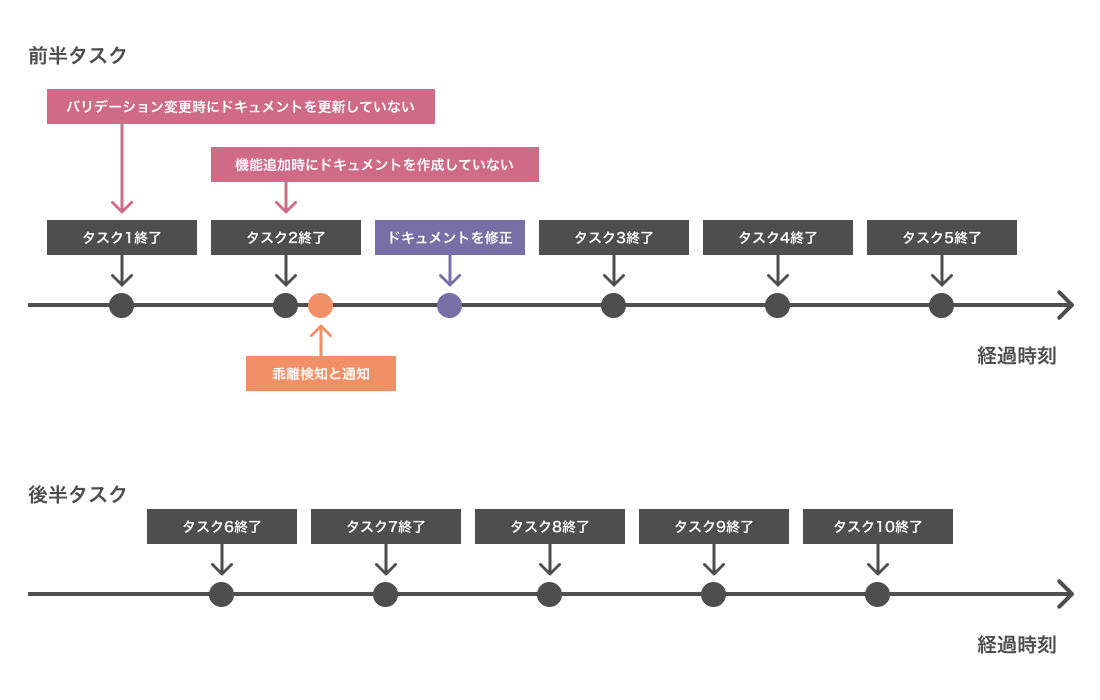
\includegraphics[width=8cm]{images/UserA.png}
    \caption{前半に提案ツールを使用した実験協力者の行動と乖離検知の流れ}
    \label{usera}
\end{figure}

実験協力者Aは,タスク1ではドキュメントを更新せずにソースコードの追加のみを行っていた.
このとき,提案ツールではバリデーションの変更からSwagger形式のドキュメントとソースコードの乖離を検知することができないため,
乖離検知を行わず,通知を送ることはなかった.
次に,新たな機能を作成するタスク2を終えたときに,提案ツールが乖離検知を行ったため,実験協力者Aに「[C1]: ドキュメントに無い機能であるget\_users を作成しています」と通知を送った.
図\ref{notification1}は,実際に実験協力者Aに通知を行った時のメッセージである.

\begin{figure}[H]
    \centering
    
\includegraphics[width=10cm]{images/notification1.png}
    \caption{乖離検知をしたときに実験協力者Aに通知を送ったときのメッセージ}
    \label{notification1}
\end{figure}

その後の後半タスクでは,前半に乖離検知の通知を受け取ったことを受けて,タスクに取り組むときは,ドキュメントとソースコードの両方を追加・修正しており,
ドキュメントとソースコードが乖離することはなかった.

\subsection{後半に提案ツールを使用した実験協力者}
後半に提案ツールを使用した実験協力者(以下,実験協力者Bと呼ぶ)の行動と乖離検知の流れを図\ref{userb}に示す.
\begin{figure}[H]
    \centering
    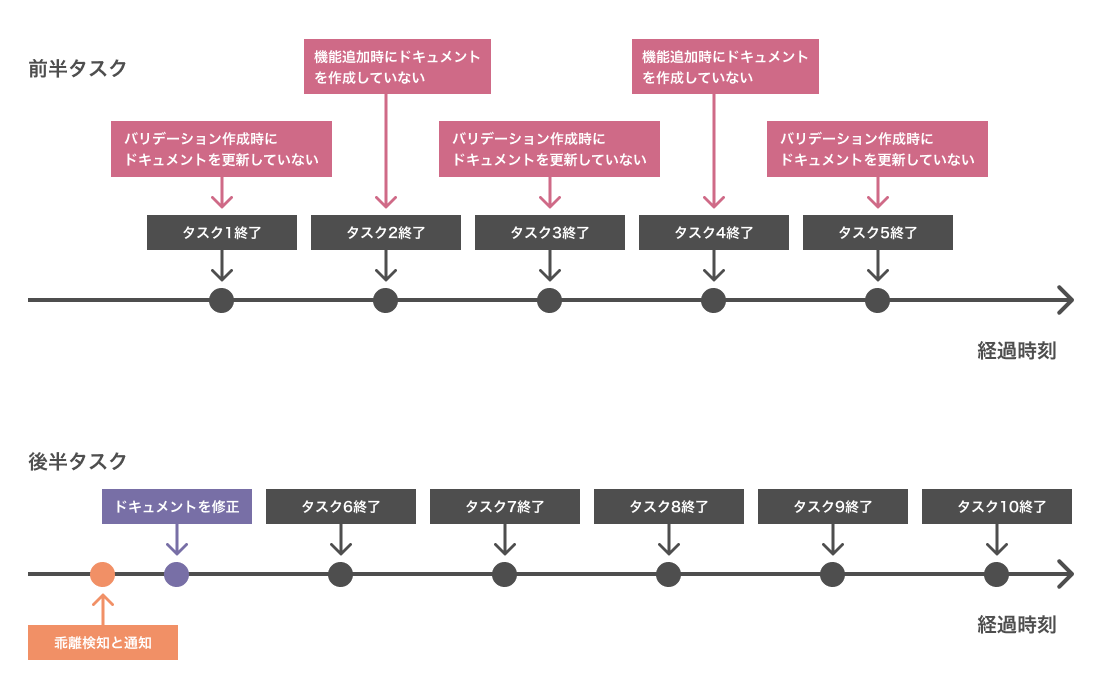
\includegraphics[width=8cm]{images/UserB.png}
    \caption{後半に提案ツールを使用した実験協力者の行動と乖離検知の流れ}
    \label{userb}
\end{figure}

実験協力者Bは,前半タスクをこなす間,一度もドキュメントに触れることなくソースコードの追加を行っていた.
後半タスク開始時に,ドキュメントとソースコードの乖離検知が行われたため,実験協力者Bに「[C1]: ドキュメントに無い機能であるget\_user get\_users\_child を作成しています」と通知を送った.
図は\ref{notification2},実際に実験協力者Bに通知を行った時のメッセージである.

\begin{figure}[H]
    \centering
    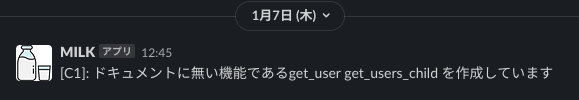
\includegraphics[width=10cm]{images/notification2.png}
    \caption{乖離検知をしたときに実験協力者Aに通知を送ったときのメッセージ}
    \label{notification2}
\end{figure}

ここで,タスク6を開始する前に,実験協力者Bはドキュメントの更新を行ったため,ドキュメントとソースコードの乖離が抑制された.
その後,後半タスクが終了するまでドキュメントとソースコードが乖離することはなかった.

\subsection{実験結果の考察}
上記では実験協力者2名について,それぞれのタスクの取り組みや,ドキュメントとソースコードの乖離検知をしたときの行動を詳細にまとめた.
2名とも,乖離検知の通知を受け取った直後に,ドキュメントの修正を行っており,全タスク終了時にはドキュメントとソースコードが乖離することはなかった.
このことから,RESTful APIの開発において,提案ツールはドキュメントとソースコードの乖離抑制に一定の効果が見込めることが判明した.
一方で,実験協力者Aのタスク1において,バリデーションを修正したがドキュメントを更新しなかったことについて,
乖離を検知できなかったため,提案ツールの性能を向上させる必要があると考えられる.

\section{アンケート結果と考察}
実施したアンケートを付録\ref{survey}に示す.
実験協力者2名に対し,Slackからの通知を受け取ったことで,ドキュメントを更新しないといけないと感じたかという質問に対し,1名が「とても思った」,1名が「やや思った」と回答した.
回答結果を図\ref{q1}に示す.
\begin{figure}[H]
    \centering
    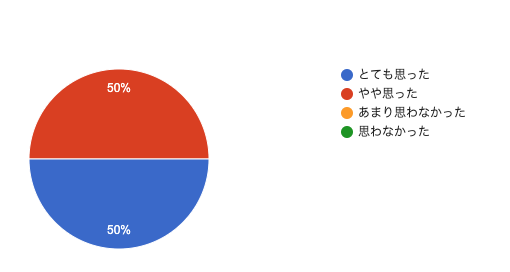
\includegraphics[width=10cm]{images/q1.png}
    \caption{アンケート結果: Slackからの通知を受け取ったことで,ドキュメントを更新しないといけないと感じたか}
    \label{q1}
\end{figure}

また,ドキュメントの更新を忘れてしまったとき,通知は必要だと感じるかという質問に対し,2名が必要であると回答した.
回答結果を図\ref{q2}に示す.
\begin{figure}[H]
    \centering
    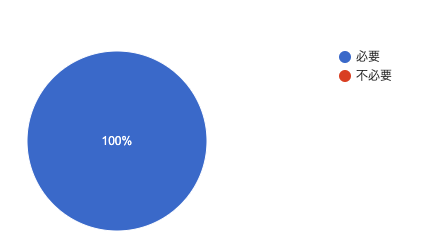
\includegraphics[width=10cm]{images/q2.png}
    \caption{アンケート結果: ドキュメントの更新を忘れてしまったとき,通知は必要だと感じるか}
    \label{q2}
\end{figure}

Slackから受け取った通知内容で改善して欲しいところはあるかという質問に対して,以下のような回答を得た.
\begin{itemize}
    \item 通知内容が簡素に感じた
    \item もっと詳細を教えて欲しい
\end{itemize}

以上のアンケート結果より,提案ツールはドキュメントとソースコードの乖離の抑制に効果を感じていることがわかった.
一方で,通知内容を改善し,開発者に親しみやすいように改良を加えることで,より使いやすいツールになることが判明した.
\chapter{結論}
本研究では,ドキュメントとソースコードの乖離の可能性のある箇所を特定および通知を行うことのできるツールの開発を行った.
ドキュメントとソースコードが乖離してしまう原因は,ビジネス要求を素早く実現することが求めらるソフトウェア開発現場において,
ソースコードの追加・修正に追われてしまい,ドキュメントの追加・修正を忘れてしまうことにあると考えた.
そこで,ドキュメントとソフトウェアの乖離の可能性のある箇所を特定および通知を行い,
ドキュメントの追加・修正を開発者に促すことでドキュメントとソースコードの乖離を抑制できると考えた.
また,開発スピードを落とさないためにも,ライブラリやフレームワーク,エディタへの制限を少なくし,既存のソフトウェア開発プロジェクトに無理なく組み込むことができる必要があると考えた.

今回提案したツールの効果を検証するために,Gitのコミット履歴を用いたシミュレーションおよび実験協力者に提案ツールを使用してもらい実験を行った.
シミュレーションの結果から,ドキュメントとソースコードの乖離リスクが検知されたときに通知を出すことで,乖離の抑制に役立つ可能性があることが判明した.
一方で,精度の高い検知を行うためには,さらなる改善を加えないといけないことがわかった.

実験では,前半5個,後半5個の合計10個のタスクを2名の実験協力者にこなしてもらい,前後半のいずれかで提案ツールが動作するように設定した.
実験の結果,前半に提案ツールを使用した実験協力者は,前半のタスクを2つこなした後に,提案ツールから乖離検知の通知を受け取った.
この後,実験協力者がドキュメントの修正を行ったため,前半タスク終了時にはドキュメントとソースコードの乖離が抑制された.
また,提案ツールを使用しない後半タスク終了時には,前半タスクで乖離したことを踏まえて作業を行ったため,ドキュメントとソースコードが乖離することはなかった.
後半に提案ツールを使用した実験協力者は,前半タスク終了時までにドキュメントを追加・修正することがなかった.
しかし,後半タスク開始時に乖離検知の通知を受け取った後に,ドキュメントの修正を行い,後半タスク終了時にはドキュメントとソースコードが乖離することはなかった.
実験協力者2名の実験終了後にドキュメントとソースコードが乖離していなかったことから,ドキュメントとソースコードの乖離リスクを検知した際に通知を行うことで,ドキュメントを修正しなくてはならないことに気づくことができるため,
提案ツールは乖離リスクの抑制に期待できることが判明した.
今後の課題として,様々なプログラミング言語の対応や,汎用性の向上,より正確な乖離リスクの特定を行う必要がある.

\end{document}